\section{Unknown Unknowns}
\label{sec:unknowns}
In order to provide a detailed discussion of unknown unknowns in the context of a predictive model, it is first necessary to formalize the concepts we will be discussing. Let $x$ represent an example belonging to some problem space $X$. In classification settings, $x$ has a ``true'' label, $\bar{y}$ from some set of possible labels $Y$. The task of a classification is to construct some predictive model, $f(x)$, that can estimate a label for each incoming example ($y = f(x)$) such that the estimated label $y$ mirrors the (usually hidden) true label, $\bar{y}$, as closely as possible. In this work, we are concerned only with models that output a posterior probability estimate over the set of available labels, that is, $p(y | x) = f(x)$. Such probabilities can then be used to select a preferred label, for instance by choosing the $y$ with the highest probability, or in the cost-sensitive setting, choosing the example with the least expected cost~\cite{elkan:2001cost}. Note that the focus on models that produce probability estimates is without loss of generality--- there exists a variety of techniques for transforming ``hard-labeling'' models into probability estimators (see, eg.~\cite{domingos1999metacost, Platt99probabilisticoutputs}).

\begin{definition}[Known Unknown]
\label{def:ku}
Let $M(x) = 1-p(\hat{y} | x)$, where $\hat{y} = \arg \max_y p(y | x)$, the class with the greatest expected posterior. Let $\epsilon \in [0,1]$ be some confidence threshold denoting a  radius from the decision boundary. Let $x'$ be an example with $M(x') \leq \epsilon$. $x'$ is said to be a ``Known unknown'' if for $x'$, $\hat{y} \neq \bar{y}$.
\end{definition}

Known unknowns as described in Definition~\ref{def:ku} corresponds to a commonly occurring notion in machine learning. The $\epsilon$-radius around the decision boundary corresponds to an ``uncertainty'' region, an area where the predictive model is unsure of itself, and where mistakes are likely to be made. This concept has been exploited in a variety of contexts, for instance, when applied to the problem of gathering labels for the purpose of model training, selecting those examples within an $\epsilon$-radius of the decision boundary corresponds to uncertainty sampling, perhaps the most well known active learning heuristic~\cite{lewis94sequential}.

Used in prediction time, the ``region of uncertainty'' around the decision boundary has been used to identify those examples where prediction should be deferred. Classification with a ``reject option'' is an extension of traditional classification where in addition to labeling each example with some $y \in Y$, a predictive system may additionally defer prediction, either by ignoring an example entirely, or perhaps sending the example to a domain expert for manual evaluation~\cite{chow:57,chow:70}. Given that such ``rejection'' likely comes at some non-trivial cost $q(x)$, the task of classification with a reject option is then to balance the expected misclassification costs with the costs of rejection.

Formally, let $\mbox{cost}(y^k | y^j)$ encode the penalty for predicting $f(x) = y^k$ when in fact the true label for $x$ is $y^j$. In this case, based on the posterior probability estimates generated by $f(x)$, a model should ideally choose the $y^k$ that minimizes the expected misclassification cost: $$L(x, y^k) = \sum_{y' \in Y} p(y = y' | x) \mbox{cost}(y^k | y')$$

Imagine for simplicity, the setting with balanced misclassification costs, that is, w.l.o.g., $\mbox{cost}(y^k | y^j) = 1$ whenever $y^k \neq y^j$ with $0$ costs for correct label attribution.  In this case, it is straightforward to show~\cite{chow:57,chow:70} that the optimal ``reject'' policy, $\mathcal{A}$ offering a minimum reject rate for a given expected error probability (or, equivalently, minimizing the expected error probability for a given reject rate) is given by:
\vspace{-0.03in}
\begin{equation}
\mathcal{A} = \left\{ x \| \min_c \hat{p}(y = c | x) > q(x) \right\}
\label{eq:rej}
\end{equation}

\begin{figure}[hbt]
\begin{center}
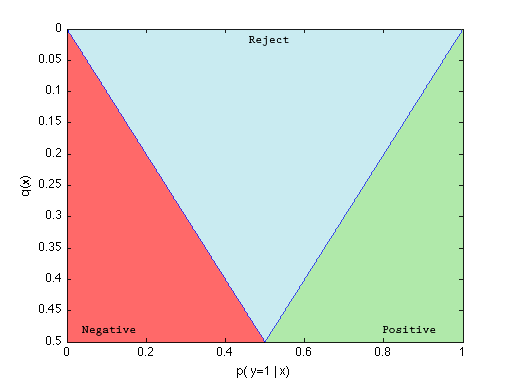
\includegraphics[width= .95 \columnwidth]{plots/reject_decision_bounds_fill.png}
\end{center}
\caption{The reject and classification regions defined by Chow's original classification with a reject option criterion defined in Equation~\ref{eq:rej}}
\label{fig:rejectdecision}
\end{figure}

As would be expected, larger query costs tend to prevent much of the efficacy of the reject option; indeed the reject option would never be exercised with $q(x)>\frac{1}{2}$. (It is optimal to always query the oracle when $q(x) = 0$, thereby yielding zero misclassification risk, assuming a perfect oracle.) Figure~\ref{fig:rejectdecision} presents the decision regions for varying query costs as a function of the posterior probability, $p(y=1|x)$. It is never advantageous to query an oracle once the costs exceed $0.5$.  Of course the uniform misclassification costs assumed by above are seldom realistic. Extending the reject rule of Chow to the case of asymmetric misclassification costs, Herbei and Wegkamp~\cite{herbei:2005} show that the optimal $\mathcal{A}$ is given by: 
\vspace{-0.03in}
\begin{equation}
\mathcal{A} = \left\{ x \| \min_{\hat{y}} L(x, \hat{y}) > q(x) \right\}
\label{eq:costrej}
\end{equation}

\begin{figure}[hbt!]
\begin{center}
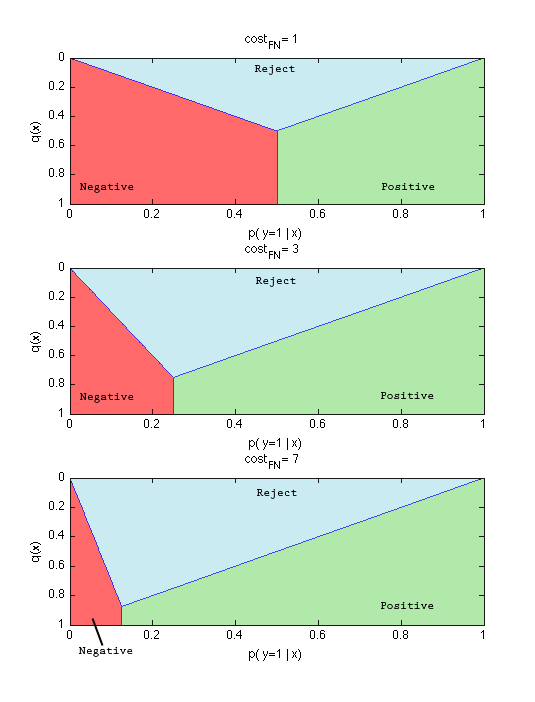
\includegraphics[width= .95 \columnwidth]{plots/cost_reject_decision_bounds_fill.png}
\end{center}
\caption{The reject and classification regions defined by Herbei and Wegkamp's misclassification cost-sensitive classification with a reject option criterion defined in Equation~\ref{eq:costrej} for different false negative costs ($\mbox{cost}_{\mbox{FN}} = \mbox{cost}(0|1)$). }
\label{fig:costdecision}
\end{figure}

As in the case of symmetric cost classification with a reject option, there are certain regions of the posterior/cost space where predictions should be rejected, and where certain labels should be chosen. Figure~\ref{fig:costdecision} presents these regions for a binary classification as a function of the posterior, $p(y=1|x)$ and of a (uniform) label cost, $q(x)$ for three different cost settings. In order to reduce the complexity of the problem being considered, we assume zero costs for correct classifications, and a false positive cost of $1$, eg. $\mbox{cost}(1|0)=1$, varying only $\mbox{cost}(0|1)$. This is equivalent to considering only the ratio of false negative to false positive costs, and re-normalizing.

In the context of classification with a reject option, ``known unknowns'' are those errors which are expected based on the confidence of the classification.  These are cases where it may be less costly to ``reject'' than to make a risky label prediction. The uncertainty radius, $\epsilon$, can be thought of as a constant $q(x)$ across all $x$.  However, while it is important to understand the mistakes that your model is known to make and to react in an appropriate manner, models in production often make mistakes far from this area of predicted uncertainty. Consider the hate speech classification system discussed previously. While deployed in a production setting, this model is likely to encounter examples eliciting a high degree of predicted uncertainty.\footnote{For instance, a encyclopedia entry discussing racial issues or a history of racism.} Those managing the model can react to these borderline examples, and perhaps build some rough estimate of a model's overall exposure to misclassification risk. However, for a variety of reasons, the model may also encounter examples where it will assign a label with high confidence, and be wrong. Call all such examples ``unknown unknowns.''

\begin{definition}[Unknown Unknown]
\label{def:uu}
Following Definition~\ref{def:ku}, let $M(x) = 1-p(\hat{y} | x)$ and let $\epsilon$ be some confidence threshold denoting a  radius from the decision boundary, with $\epsilon \in [0,1]$. In this setting, an example $x'$ is said to be an ``\emph{unknown unknown}'' if $M(x') > \epsilon$, that is, $x'$ is outside the region of uncertainty, but $\hat{y} \neq \bar{y}$, i.e., the example is misclassified but the classifier is certain that it was correctly classified.
\end{definition}

Definition~\ref{def:uu} codifies the notion of an ``unknown unknown''. Intuitively, these are examples that are distant from any decision boundary, examples that the model is quite certain a correct label can be assigned, yet are still labeled incorrectly.  While in the strict sense, the above definition includes ``random noise''---individual examples that for whatever reason do not have the expected label,\footnote{For instance,  due to erroneous labeling, signal degradation, or non-pathological difficulties in data collection.}---the motivating case is disjunctive sub-regions of the problem space~\cite{weiss10disjunct}. These are small, yet consistently labeled neighborhoods of examples isolated from the body of examples of the same class. These ``islands'' of examples may be sufficiently rare in the relative sense to avoid detection from random sampling processes used to generate training sets~\cite{attenberg:2010inactive, attprov:kdd2010}. However, their absolute size and prevalence in many real world problems makes them a genuine risk.

Figure~\ref{fig:unknown} presents a fairly typical classification
scenario that might be impacted by ``unknown unknowns''. On the top,
we see an inseparable two-class problem, with a linear decision
boundary that minimizes the prediction errors on this space. Above and
below this decision boundary, we see an example $\epsilon$-radius,
encapsulating the region where mistakes are known to occur. This
represents a typical post-training understanding of the problem space: 
data is gathered by some random process, for instance via active
learning. An imperfect model is trained, however, areas where mistakes
occur are known and expectations can be managed. On the bottom we see
a typical scenario when such models are deployed in the wild---rare
disjunctive sub-regions of the problem space emerge.  These are portions of the
problem space that escaped the initial sampling process used to generate
the training set. These unknown unknowns while small in terms of their
proportion of the problem space may still exist in large absolute
numbers.  However, because they are unobserved during model
construction, they have likely escaped any possible contingency
planning for dealing with their associated mistakes.

\begin{figure}[hbt!]

\begin{center}
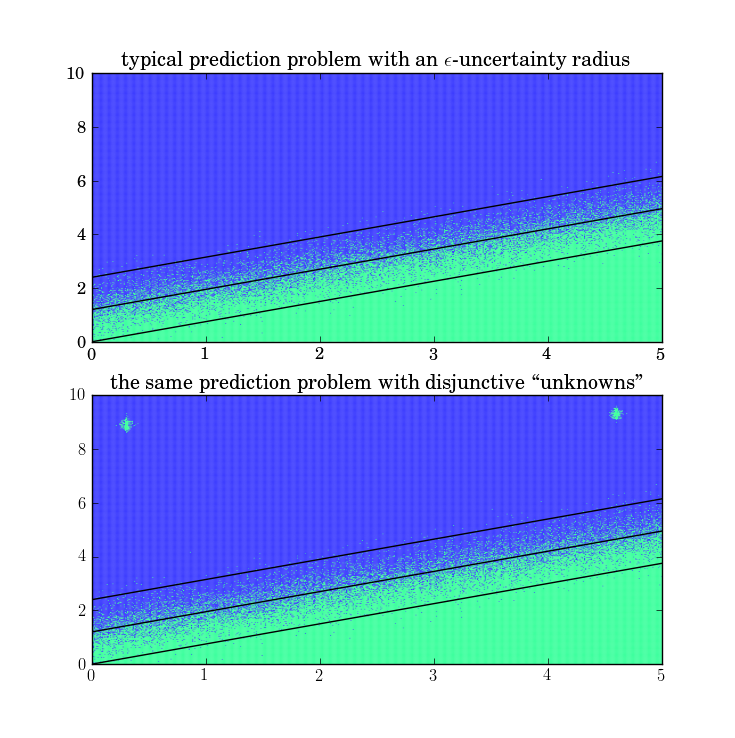
\includegraphics[width= 1.05 \columnwidth]{plots/example_function_2.png}
\end{center}
\vspace{-0.2in}
\caption{A typical classification setting. On the the top we see the decision boundary that minimizes the prediction prediction error of a inseparable training set. Additionally, we see the $\epsilon$-radius around the classifier where mistakes are though to occur. The bottom, we see the same classifier with the inclusion of small, disjunctive ``unknowns'', presenting mistakes that occur well outside a model's region of uncertainty. }
\label{fig:unknown}
\end{figure}

\josh{if i have time, go back and rephrase things in terms of cost bounds rather than probability bounds.}
